% Full instructions available at:
% https://github.com/elauksap/focus-beamertheme

\documentclass{beamer}
\usetheme{focus}

\usepackage{wrapfig}
\usepackage{csquotes}
\usepackage{listings}
\usepackage{verbatim}
\usepackage{hyperref}
\usepackage{graphicx}
\usepackage{xparse}

\AtBeginSection[]
{
  \begin{frame}
    \frametitle{Table of Contents}
    \tableofcontents[currentsection]
  \end{frame}
}

\title{Using LaTeX and Markdown for Reproducible Research}
\subtitle{}
\author{Erik Beck \\ Emily Y. Li}
\titlegraphic{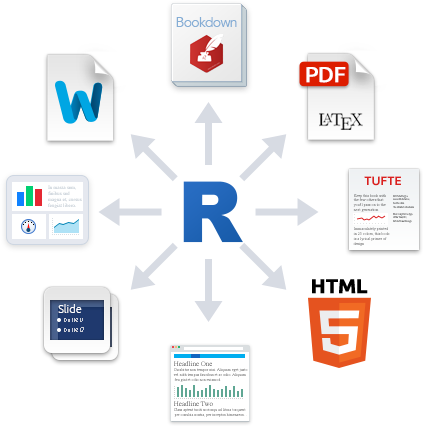
\includegraphics[width = 4.75cm]{Rlogotree.png}}
\institute{2018 US EPA \\ R User Group Workshop}
\date{11 Sept 2018}

\begin{document}
    \begin{frame}
        \maketitle
    \end{frame}
    
    \begin{frame}
        \frametitle{Table of Contents}
        \tableofcontents
    \end{frame}

\section{Agenda}

\begin{frame}{Time Frame \& Objectives}
\begin{exampleblock}{Using LaTeX and Markdown for Reproducible Research}
\begin{center}
    \begin{tabular}{c c c}
    Day & Time & Room \\
    \textbf{Tues, Sept 11} & \textbf{8:30-11:30am} & \textbf{C111C}
\end{tabular}
\end{center}
\end{exampleblock}

\begin{itemize}
    \item This 1/2-day workshop will provide attendees with hands-on experience
using the basics of LaTeX, Markdown, and the R package knitr.
    \item After attending this workshop, you will be able to use these tools to
facilitate reproducible reports and research with R.
\end{itemize}
% This would be a really good place to check that everyone has R and RStudio installed.
% Insert testing code here
\end{frame}

\begin{frame}{Steps/Agenda}
\vfill
We will try to use our three hours as effectively as possible.
\begin{exampleblock}{Rough Agenda}
%\begin{description}
%\item[8:30] System checks
%\item[8:45] Intro to LaTeX
%\item[9:00] Intro to Markdown
%\item[9:15] Markdown \& LaTeX
%\item[9:40] Reproducible Research
%\hline
%\item[9:50] \emph{BREAK}
%\hline
%\item[10:00] Dynamic documents with Sweave and knitr
%\item[10:30] Markdown \& LaTeX with R
%\end{description}
\begin{center}
\begin{tabular}{r|r|l}
    \textbf{\#} & \textbf{Time} & \textbf{Topic} \\
    1 & 8:30 & System checks \& agenda \\
    2 & 8:45 & Intro to LaTeX \\
    3 & 9:00 & Intro to Markdown \\
    4 & 9:15 & Markdown \& LaTeX examples \\
    5 & 9:40 & Reproducible Research \\
    \hline
     & 9:50 & \emph{BREAK} \\
    \hline
    6 & 10:00 & Dynamic documents with Sweave and knitr \\
    7 & 10:30 & Markdown \& LaTeX with R \\
    8 & 11:20 & Wrap-up \& additional resources
\end{tabular}
\end{center}
\end{exampleblock}
% We definitely want to go over these times before the workshop!
\end{frame}

\section{Introduction to LaTeX}
\begin{frame}{Intro to LaTeX}
\vfill
LaTeX is a tool for high-quality typesetting, designed for the production of technical and scientific documentation.
\vfill
\begin{block}{How do you pronounce ``LaTeX''?}
    \begin{quote}
        TeX is usually pronounced tech, making \emph{'lah}-teck, lah-\emph{'teck}, and \emph{'lay}-teck the logical choices; but language is not always logical, so \emph{'lay}-\emph{'tecks} is also possible.
    \end{quote}
    --- Leslie B. Lamport, original developer of \LaTeX{}
\end{block}
\end{frame}

\begin{frame}{Intro to LaTeX}
LaTeX is widely used in academia for the publication of scientific documents in many fields, including mathematics, statistics, computer science, engineering, chemistry, physics, economics, and political science.

\begin{enumerate}
    \item \textbf{TeX engines have excellent quality output.} This especially holds for complex documents such as those with many tables, figures, equations, cross-references or hyperlinks---or just with many pages.
    \item \textbf{TeX is fast.}
    \item \textbf{TeX is consistent.}
    \item \textbf{TeX is stable.} It will never eat your document. \emph{Ever.}
\end{enumerate}
\vfill
--- \url{https://www.ctan.org/tex/}
% I'd like to add that while LaTeX is most used for medium to long papers, there are also EXCELLENT templates for very good-looking short documents, like resumes.
% Add an Erik Resume version here?
\end{frame}

\begin{frame}[fragile]{LaTeX: Minimal example}
Here is a minimal example of a full document written in LaTeX.
\begin{exampleblock}{}
\begin{lstlisting}
\documentclass{article}
\title{A Minimal LaTeX Example}
\author{Emily Li}

\begin{document}
\maketitle

Yer a wizard, Harry.

\end{document}
\end{lstlisting}
\end{exampleblock}
% We will revisit this code later to make sure everyone compiled it.
\end{frame}

\begin{frame}{Levels of TeX: A disambiguation}
\begin{alertblock}{Help! There are too many words with ``TeX'' in them!}
If you are wondering, \alert{\emph{``Should I use LaTeX or MiKTeX?''}}, allow us to clear that up. These two slides will cover four types of TeX-related terms: distributions, editors, engines, and formats.
\end{alertblock}
\begin{enumerate}
    \item \textbf{Distributions:} \textit{MiKTeX, TeX Live, etc.} This is TeX-related software to be downloaded and installed. When someone says, ``I need to install TeX on my machine,'' they're usually looking for a distribution.
    \item \textbf{Editors:} \textit{Emacs, TeXworks, TeXShop, TeXStudio, etc.} These editors are what you use to create a document file. Some (e.g., TeXShop) are devoted specifically to TeX, while others (e.g., Emacs) can be used to edit any sort of file.
\end{enumerate}
\vfill
--- \url{http://www.tug.org/levels.html}
\end{frame}
\begin{frame}{Levels of TeX: A disambiguation}
\begin{exampleblock}{A quick note on editors}
You can also use Notepad to edit plaintext, including LaTeX code.
\end{exampleblock}
\begin{enumerate}
\setcounter{enumi}{2}
    \item \textbf{Engines:} \textit{TeX, pdfTeX, XeTeX, LuaTeX, etc.} These are the executable binaries which implement different TeX variants. When someone says, ``TeX can't find my fonts,'' they usually mean an engine.
    \item \textbf{Formats:} \textit{LaTeX, plain TeX, etc.} These are the TeX-based languages in which one actually writes documents. When someone says, ``TeX is giving me a mysterious error,'' they usually mean a format. (Incidentally, ``LaTeX'' has meant ``LaTeX2e'' for many years now.)
\end{enumerate}
\vfill
--- \url{http://www.tug.org/levels.html}
\end{frame}

\begin{frame}{TeX Distributions}
To compile LaTeX, your computer needs one of these TeX distributions installed:
\begin{block}{TeX Distributions}
\begin{center}
    \begin{tabular}{c l}
    Distribution & Operating System \\
    \hline
    MiKTeX & Windows OS \\
    TeX Live & Linux and other UNIX-like systems \\
    MacTeX & Mac OS X
\end{tabular}
\end{center}
\end{block}
You can also use an online ready-to-use option like \href{https://www.sharelatex.com/}{ShareLaTeX} or \href{https://www.overleaf.com/}{Overleaf}.
\end{frame}

\begin{frame}[fragile]{LaTeX: Revisiting the minimal example}
\begin{exampleblock}{Try compiling this LaTeX}
\begin{lstlisting}
\documentclass{article}
\title{A Minimal LaTeX Example}
\author{Emily Li}

\begin{document}
\maketitle

Yer a wizard, Harry.

\end{document}
\end{lstlisting}
\end{exampleblock}
\end{frame}

\section{Introduction to Markdown}
\begin{frame}{Intro to Markdown}
\begin{columns}[t, onlytextwidth]

\column{0.5\textwidth}
\vfill
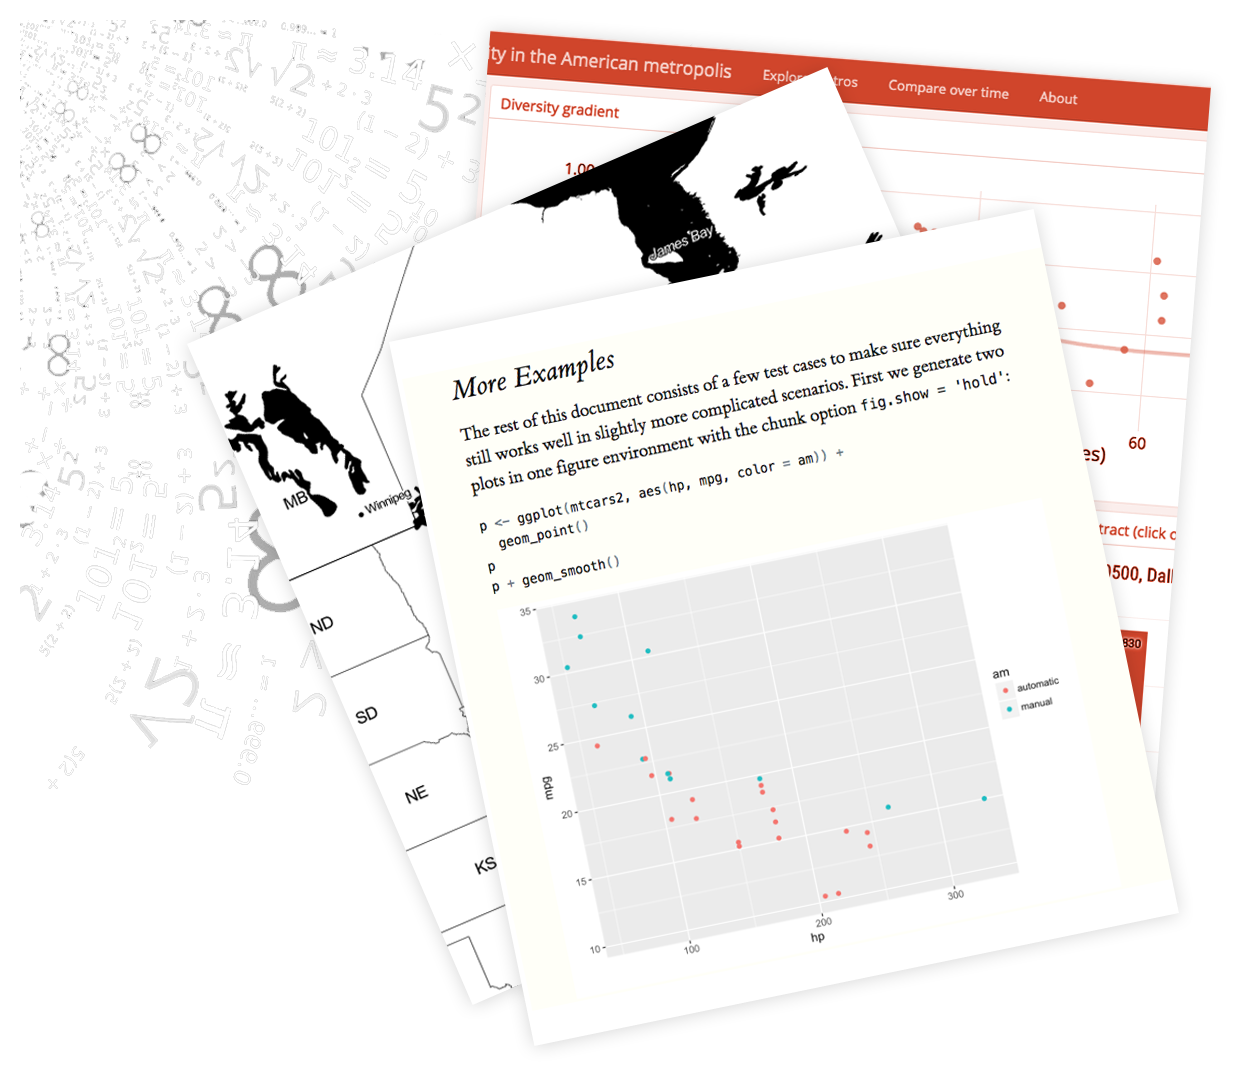
\includegraphics[width=\textwidth]{markdown-examples.png}
\vfill
{\footnotesize \url{https://rmarkdown.rstudio.com/}}

\column{0.5\textwidth}
    \begin{itemize}
        \item An \textbf{.Rmd file} is an R Markdown file
        \item Contains the code that a scientist needs to reproduce your work, along with the narration that a reader needs to understand it.
        \item Choose to export the finished report in a variety of formats, including HTML, PDF, or MS Word.
    \end{itemize}

\end{columns}
\end{frame}

\begin{frame}{Intro to Markdown}
\begin{itemize}
    \item Markdown allows us to write using an easy-to-read, easy-to-write plain text format.
    \item As long as you know how to write emails, you can learn it in a few minutes.
    \item \url{https://en.wikipedia.org/wiki/Markdown\#Example}
\end{itemize}
\vfill
\begin{alertblock}{Limitations of Markdown}
Markdown was primarily designed to be simple. \\ For more complicated typesetting, LaTeX may be preferred.
\end{alertblock}
\vfill
\end{frame}


\begin{frame}{Uses for Markdown}
% EHB
  \begin{itemize}
  \item Maximal focus on content, minimal focus on formatting while writing.
  \item Quick layout of documents.
  \item Can be converted to a variety of formats easily (Pandoc, others).
  \item Format durability (records)
  \end{itemize}
\end{frame}

\begin{frame}[fragile]{Intro to Markdown}
\begin{exampleblock}{A short example of Markdown}
  % Made changes so standalone pandoc will work.
  % See mark-list-example.md in the same directory as this file
  \begin{lstlisting}
# First level header

Sup universe!

## Second level header

This is **bold**, and _italic_.

- list item
- list item

You can write an ordered list:

1. item 1
1. item 2 # this line will render as "2."
\end{lstlisting}
\end{exampleblock}
\end{frame}

\begin{frame}{Workflow in Markdown}
Using RStudio:
\begin{description}
\item[Open] a new .Rmd file, which pre-populates with a template
\item[Write] a document by editing the template
\item[Knit] the document to create a report; use the knitr button or render() to knit
\item[Preview] output in IDE window
\item[Publish] to web server (optional)
\item[Use] output file that is saved alongside .Rmd
\end{description}
\vfill
Helpful link: \\ \url{https://rmarkdown.rstudio.com/lesson-2.html}
\end{frame}

\section{Markdown \& LaTeX examples}


\section{Reproducible Research}
\begin{frame}[noframenumbering]{Reproducible Research}
\begin{center}
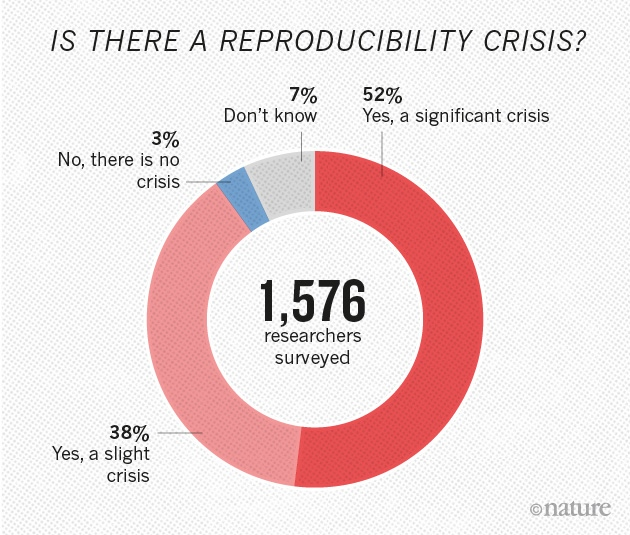
\includegraphics[width=.82\textwidth]{nature-reproducibility-graphic.jpeg}
\end{center}
\vspace{-0.5cm}
{\footnotesize \href{https://www.nature.com/news/1-500-scientists-lift-the-lid-on-reproducibility-1.19970}{\textit{Nature} \textbf{533}, 452-454 (26 May 2016) | doi:10.1038/533452a}}
\vfill
\end{frame}

\begin{frame}[noframenumbering]{Reproducible Research}
    \begin{center}
        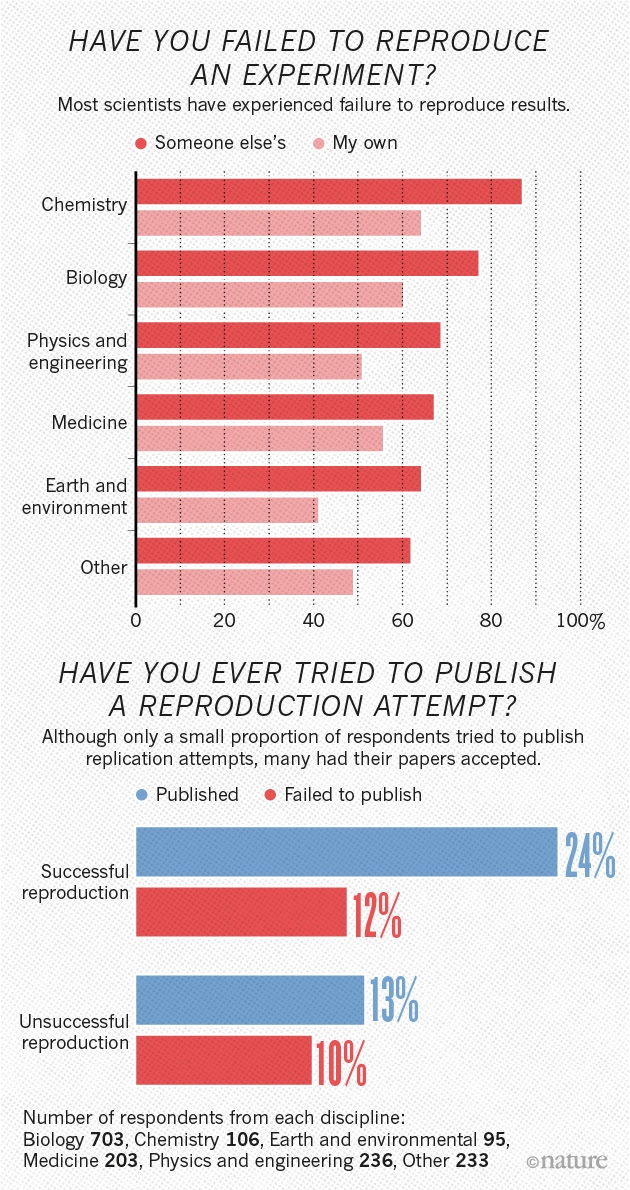
\includegraphics[trim=0 550 0 15, clip, width=.71\textwidth]{nature-reproducibility-breakdown.jpg}
    \end{center}
\vspace{-0.5cm}
{\footnotesize \href{https://www.nature.com/news/1-500-scientists-lift-the-lid-on-reproducibility-1.19970}{\textit{Nature} \textbf{533}, 452-454 (26 May 2016) | doi:10.1038/533452a}}
\vfill
\end{frame}

\begin{frame}{Reproducible Research}
\begin{alertblock}{Results must be reproducible to be trustworthy.}
\begin{quote}
    An article about computational science in a scientific publication is not the scholarship itself, it is merely the advertising of the scholarship. The actual scholarship is the complete software development environment \textbf{and the complete set of instructions which generated the figures}.
\end{quote}
\end{alertblock}
--- 1995, David L. Donoho, professor of statistics at Stanford University
\vfill
    % Though Donoho was referring to computational science, journals in other data-driven fields such as biostatistics have been moving in the direction of reproducible research as well.
    % This would be a good time to quickly discuss attendees' difficulties with reproducing research.
\end{frame}
    
\begin{frame}[fragile]{Reproducible Research}
This chunk of R code produces a figure that illustrates a simulation of Brownian motion for 100 steps.
        \begin{exampleblock}{Try running this in RStudio}
\begin{lstlisting}
set.seed(1213) # for reproducibility
x <- cumsum(rnorm(100))
plot(x, type = "l",
     ylab = expression(x[i+1]==
                       x[i]+epsilon[{i+1}]),
     xlab = "step")
\end{lstlisting}
        \end{exampleblock}
\end{frame}

\begin{frame}[fragile]{Reproducible Research}
%        \begin{exampleblock}{}
%\begin{lstlisting}
%set.seed(1213)
%x <- cumsum(rnorm(100))
%plot(x, type = "l",
%     ylab = expression(x[i+1]==x[i]+epsilon[{i+1}]),
%     xlab = "step")
%\end{lstlisting}
%        \end{exampleblock}
\begin{center}
    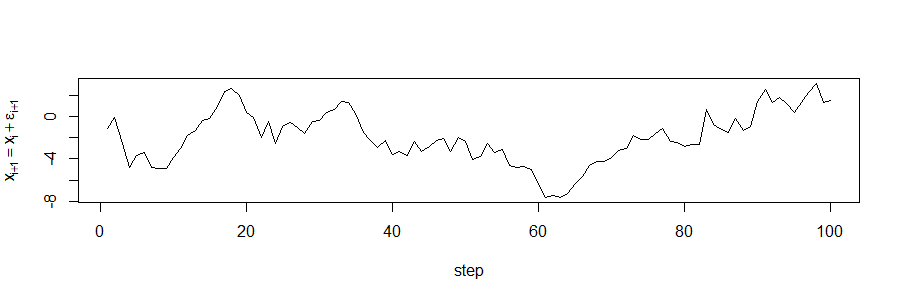
\includegraphics[width=\textwidth]{Brownian-motion.png}
\end{center}
To put this into a document by hand, we would have to open RStudio, compile the code to draw the plot, save it as an image, then insert it into a document with \verb|\includegraphics{}|.
\vfill
Then what if we want to change the random seed in \verb|set.seed()|, or the y-axis label?
% This is both tedious and difficult for the author to maintain. If we want to change the figure, we have to update both the source code and the typesetting file.
\vfill
\end{frame}

\begin{frame}{Dynamic report generation}
\vfill
\begin{itemize}
    \item Instead of separating the results from the computation, we can put everything in one document.
    \item When we compile this document, the computation will be executed, giving us the results directly.
    \item Integrating code with narratives is not only easier, but also provides details needed for reproducibility. % It does not guarantee RR, but it is an important step towards RR. RR is one possible by-product of dynamic documents.
    \vfill
    \begin{exampleblock}{Dynamic documents are easier than cut-and-paste}
    It is fairly common to see student homework and exercises among the countless user contributions on \href{https://rpubs.com/}{RPubs}. Once students are trained, we may expect more reproducible scientific research in the future. % Easy tools promote RR very quickly.
    \end{exampleblock}
    \vfill
\end{itemize}
% We should not expect all reports in the world to be publicly available, but it is better to share even mediocre or flawed code or problematic datasets than to not share anything at all. 
\end{frame}

\begin{frame}{Dynamic documents---a short example}
This table shows a subset of the $mtcars$ dataset.

\begin{center}
\begin{tabular}{lrrrrrr}
      & mpg & cyl & disp & hp & drat & wt \\
    Mazda RX4 & 21.0 & 6 & 160 & 110 & 3.90 & 2.620 \\
    Mazda RX4 Wag & 21.0 & 6 & 160 & 110 & 3.90 & 2.875 \\
    Datsun 710 & 22.8 & 4 & 108 & 93 & 3.85 & 2.320 \\
    Hornet 4 Drive & 21.4 & 6 & 258 & 110 & 3.08 & 3.215 \\
    Hornet Sportabout & 18.7 & 8 & 360 & 175 & 3.15 & 3.440 \\
    Valiant & 18.1 & 6 & 225 & 105 & 2.76 & 3.460 \\
\end{tabular}
\end{center}

Have you ever included a table in your document? In LaTeX, the code would look like this\ldots
\end{frame}

\begin{frame}[fragile]{Dynamic documents---a short example}
    \begin{exampleblock}{Manual table in LaTeX}
    \begin{lstlisting}
\begin{tabular}{lrrrrrr}
      & mpg & cyl & disp & hp & drat & wt \\
    Mazda RX4 & 21.0 & 6 & 160 & 110 & 3.90 & 2.620 \\
    Mazda RX4 Wag & 21.0 & 6 & 160 & 110 & 3.90 & 2.875 \\
    Datsun 710 & 22.8 & 4 & 108 & 93 & 3.85 & 2.320 \\
    Hornet 4 Drive & 21.4 & 6 & 258 & 110 & 3.08 & 3.215 \\
    Hornet Sportabout & 18.7 & 8 & 360 & 175 & 3.15 & 3.440 \\
    Valiant & 18.1 & 6 & 225 & 105 & 2.76 & 3.460 \\
\end{tabular}
    \end{lstlisting}
    \end{exampleblock}
Even if you maintain this table in Excel, there are manual steps and human intervention required to update your document.
\end{frame}

\begin{frame}[fragile]{Dynamic documents---a short example}
%\vfill
If you wanted to include this same table in your dynamic document, you would only need this code:
    \begin{exampleblock}{Table generated in R code}
    \begin{lstlisting}
library(knitr)
kable(head(mtcars[, 1:6]))
    \end{lstlisting}
    \end{exampleblock}
If you ever update the \verb|mtcars| dataframe, the table will update in the document on its own.
%\vfill
%\begin{quote}
%    ``The source code is real.'' --- Data analysis philosophy
%\end{quote}
%\vfill
\end{frame}

\begin{frame}[focus]
    Break for 10 minutes
    
    \vfill
    
\includegraphics[trim=100 0 100 0, clip, width=\textwidth]{stretching-work.png}
    \vspace{-0.7cm}
    {\tiny Image source \url{https://getcubefit.com/}. Not an endorsement of the company.}
\end{frame}

\begin{frame}[focus]
    Welcome back!
\end{frame}

\section{Dynamic documents with Sweave and knitr}

\begin{frame}{Sweave and knitr}
    \textbf{Sweave} and \textbf{knitr} can compile narrative documents with R code.
    \vspace{0.5cm}
    \begin{description}
    \item[Sweave] is included in base R, and specifically compiles R code integrated into LaTeX or LyX documents.
    \item[knitr] compiles any input language (R, Python, SAS\ldots) inside any markup language (LaTeX, Markdown, HTML\ldots)
    \end{description}
\end{frame}

\begin{frame}[fragile]{Sweave}
    \vfill
    \textbf{Sweave} has been a prominent, longstanding tool for dynamic documents since 2002.
    \begin{itemize}
        \item Combines the power of R with the production value of LaTeX
        \item Part of base R (as the \verb|Sweave()| function)
        \begin{itemize}
            \item From your R session: \verb|Sweave("your_file.Rnw")|
            \item From the command line: \verb|R CMD Sweave your_file.Rnw|
        \end{itemize}
    \end{itemize}
    \vfill
    However\ldots
    \begin{itemize}
        \item Development has plateaued in recent years
        \item Not modular enough; extensions may become incompatible. Some packages are no longer synchronized.
        \item A PDF produced from LaTeX looks great, but is often not the format we need when collaborating.
        %\item LaTeX (to produce Rnw documents) is more complicated than RMarkdown (Rmd), and documents rarely need to be produced as PDFs unless submitting a manuscript to journals.
    \end{itemize}
    \vfill
\end{frame}

\begin{frame}{knitr}
\vfill

\textbf{knitr} was largely motivated by Sweave, and designed to be easier to maintain and extend.

\begin{block}{}
% The design of knitr allows any input languages (e.g. R, Python and awk) and any output markup languages (e.g. LaTeX, HTML, Markdown, AsciiDoc, and reStructuredText)
\begin{quote}
    The design of knitr allows any input languages and any output markup languages.
\end{quote} --- \href{https://yihui.name/knitr/}{Yihui Xie, creator of knitr}
\end{block}

\begin{itemize}
    \item Can compile code in Markdown documents, which are intuitive and human-readable for formatting. % Even someone who has never heard of Markdown can understand what is happening to some extent.
    \item Works very well with Pandoc, so creating a Word document or OpenDocument format is just as easy as creating a PDF.
\end{itemize}

\vfill

{\small Check out \url{https://www.rdocumentation.org/packages/knitr} for more info on installation, motivation, usage, and functions.}

%First of all, knitr uses Rmarkdown, a set of intuitive human-readable code to do the formatting. While LaTeX is by no means as complicated as its reputation seems to suggest, Rmarkdown is actually easy. By human-readable I mean that anyone who has never even heard of Rmarkdown can understand what is happening to some extent.
%Sweave is great for producing PDF, but that’s one of the biggest drawbacks of LaTeX in the social sciences: while the PDF may look good, they are not the format we need when collaborating with Word-only colleagues, and with rare exceptions when submitting a manuscript to journals. Knitr works very well with Pandoc, so creating a Word document or an ODF is just as easy as creating a PDF. The other day I had to submit a supplementary file as a *.doc file, even though it’ll end up as a PDF on Dataverse or so. With knitr this didn’t take long.
%knitr supports R, Python, Ruby, Haskell, awk/gawk, sed, shell scripts, Perl, SAS, TikZ, Graphviz, C++, and more. 
\end{frame}

\begin{frame}[fragile]{Setting up knitr}

    \begin{exampleblock}{Install knitr}
    \begin{lstlisting}
install.packages('knitr', dependencies = TRUE)
    \end{lstlisting}
    \end{exampleblock}

Go to the menu $Tools~>~Options~>~Sweave$ and switch the default option for weaving (compiling) to \textbf{knitr}. 
\vfill
{\small Visit \url{https://yihui.name/knitr/faq/} for frequently asked questions.}
\end{frame}

\section{Markdown \& LaTeX with R}

\begin{frame}{Markdown \& LaTeX side-by-side}
    \begin{center}
        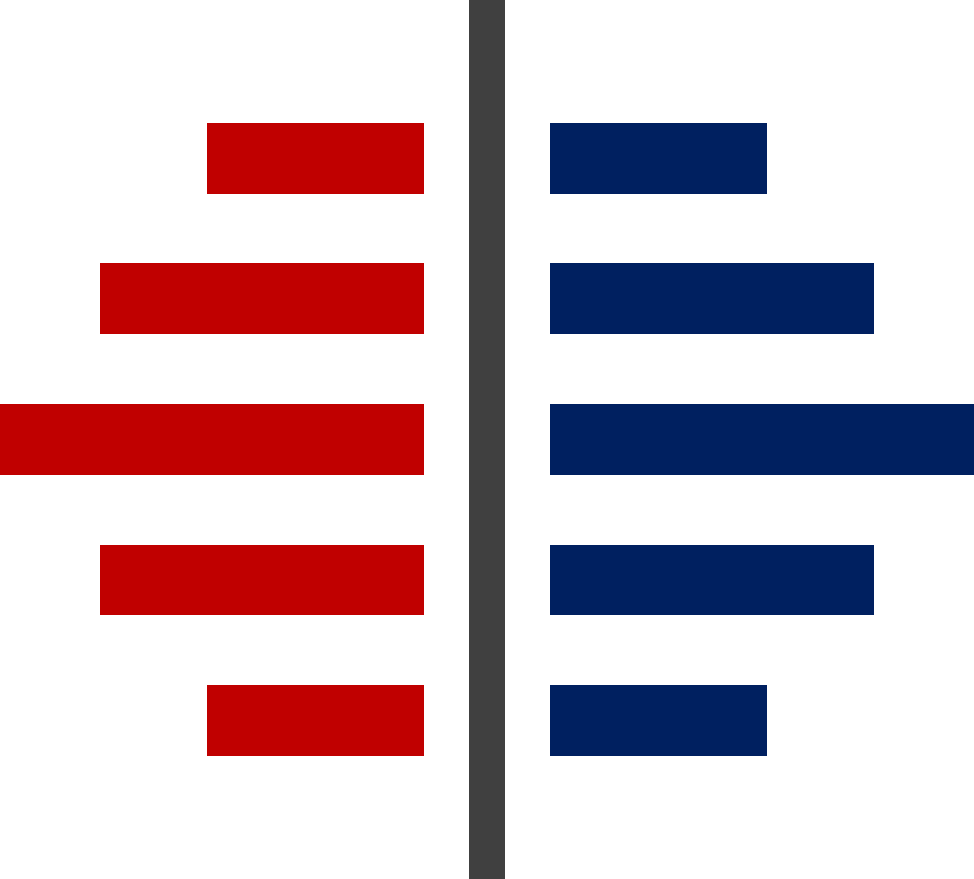
\includegraphics[width=0.4\textwidth]{comparison.png}
    
    We'll look at a side-by-side comparison of \\ Markdown and LaTeX using the exact same analysis.
    
    \vfill
    
    We will be using RStudio to edit and \\ compile the source code.
    
    \vfill
    \end{center}
        % You could also use Emacs or LyX, or other editors you have configured yourself.
    % Using dedicated editors just makes it easier to input code chunks and call knitr.
\end{frame}

%\begin{frame}[fragile]{Example LaTeX with analysis}
%\begin{lstlisting}
%\documentclass{article}
%\begin{document}
%\title{Speed and Stopping Distance}
%\author{Yihui Xie, creator of knitr}
%\maketitle
%
%We examine the relationship between speed and stopping distance using a linear regression model:
%$Y = \beta_0 + \beta_1 x + \epsilon$.
%
%<<model, fig.width=4, fig.height=3, fig.align='center'>>=
%par(mar = c(4, 4, 1, 1), mgp = c(2, 1, 0), cex = 0.8)
%plot(cars, pch = 20, col = 'darkgray')
%fit <- lm(dist ~ speed, data = cars)
%abline(fit, lwd = 2)
%@
%
%The slope of a simple linear regression is \Sexpr{coef(fit)[2]}.
%
%\end{document}
%\end{lstlisting}
%\end{frame}

\begin{frame}[focus]
    Demo $Rnw-input.Rnw$
    % The chunk options in this example specify the plot size to be 4 by 3 inches, and plots should be aligned in the center.
\end{frame}

\begin{frame}{R in LaTeX}
\vfill
    \begin{itemize}
        \item Files that mix R code and LaTeX have file extension \textbf{.Rnw}
        \item When embedding R code in an Rnw document, start a code chunk with $<<>>=$ and terminate it with $@$.
        \item Write chunk options in between $<<$ and $>>=$
    \end{itemize}
\vfill
\begin{block}{Oh, so now the file isn't ``.TeX'' anymore?}
``Rnw'' stands for ``R no web''. \href{https://www.cs.tufts.edu/~nr/noweb/}{NoWeb} is an old but still active simple system for mixing code and narratives.
\end{block}
\end{frame}

%\begin{frame}[fragile]{Example Markdown with analysis}
%\begin{lstlisting}
%---
%title: Speed and Stopping Distance
%---
%
%We examine the relationship between speed and stopping distance using a linear regression model:
%$Y = \beta_0 + \beta_1 x + \epsilon$.
%
%```{r fig.width=4, fig.height=3, fig.align='center'}
%par(mar = c(4, 4, 1, 1), mgp = c(2, 1, 0), cex = 0.8)
%plot(cars, pch = 20, col = 'darkgray')
%fit <- lm(dist ~ speed, data = cars)
%abline(fit, lwd = 2)
%```
%
%The slope of a simple linear regression is `r coef(fit)[2]`.
%\end{lstlisting}
%\end{frame}

\begin{frame}[focus]
    Demo $Rmd-input.Rmd$
\end{frame}

\begin{frame}{R in Markdown}
\vfill
\begin{itemize}
    \item $```\{r\}$ opens a code chunk and $```$ terminates a code chunk
    \item Inline R code is written in backticks $`~`$
    \item Chunk options are written before the closing brace $\}$ in the chunk header
    \item By comparison, Markdown has simpler commands.
\end{itemize}
\vfill
\begin{exampleblock}{You had me at ``keyboard shortcut''}
In RStudio, for either $.Rnw$ or $.Rmd$, quickly insert code chunks with the keyboard shortcut $Ctrl + Alt + I$.
% For OS X, use $Command + Option + I$.
\end{exampleblock}
\vfill
\end{frame}

\begin{frame}[fragile]{Quick reporting in Markdown}
    It is also possible to generate a quick report from R script using \textbf{knitr}'s \verb|stitch()| function.
    \begin{exampleblock}{Stitch a quick report}
    \begin{lstlisting}
    library(knitr)
    stitch("your-script.R")
    \end{lstlisting}
    \end{exampleblock}
    \begin{itemize}
        \item \verb|stitch()| provides a template so the user only feeds the template with one R script and knitr will compile the template to a report.
        \item Currently it has built-in templates for LaTeX (default), HTML, and Markdown.
    \end{itemize}
    {\small See \verb|?stitch| for details.}
\end{frame}

\begin{frame}{R in Markdown \& LaTeX}
    \vfill
    \begin{center}
        Thoughts?
    \end{center}
    \vfill
    \begin{description}
    \item[Markdown] is super easy to learn (\textit{i.e.} there's nothing TO learn), but is very limited in typesetting controls.
    \item[LaTeX] has more commands to learn, but always looks better---even with minimal coding.
    \end{description}
    \vfill
    Each serves a different purpose. If you're writing a journal article, thesis, textbook, or r\'esum\'e, you may want the extra precision.
    %\vfill
    %Also, \textbf{you can use them both at the same time}. Theoretically. I haven't tried this. Might be an advanced technique.
    
    % This would be a good slide to leave up while working through demos.
    \vfill
\end{frame}

%\begin{frame}{Yer a wizard, Harry}
%    This would be a slide for calling to pandoc to get an Rmd file into a LaTeX document. If I get that to work.
%\end{frame}

%\begin{frame}{Markdown and LaTeX syntax summary}
%    \begin{block}{A syntax summary of R LaTeX and R Markdown document formats.}
%    \begin{tabular}{l|l|l|l}
%        Format & Start chunk & End chunk & Inline code \\
%        \hline
%        Rnw & <<*>>= & @ & \begin{lstlisting}\Sexpr{x}\end{lstlisting} \\
%        Rmd & ```{r *} & ``` & `r x`
%    \end{tabular}
%    \end{block}
%\end{frame}

%    \begin{frame}[plain]{Plain frame}
%        This is a frame with plain style and it is numbered.
%    \end{frame}
    
%    \begin{frame}[t]
%        This frame has an empty title and is aligned to top.
%    \end{frame}
    
%    \begin{frame}[noframenumbering]{No frame numbering}
%        This frame is not numbered and is citing reference \cite{knuth74}.
%    \end{frame}
    
%    \begin{frame}{Typesetting and Math}
%        The packages \texttt{inputenc} and \texttt{FiraSans}\footnote{\url{https://fonts.google.com/specimen/Fira+Sans}}\textsuperscript{,}\footnote{\url{http://mozilla.github.io/Fira/}} are used to properly set the main fonts.
%        \vfill
%        This theme provides styling commands to typeset \emph{emphasized}, \alert{alerted}, \textbf{bold}, \textcolor{example}{example text}, \dots
%        \vfill
%        \texttt{FiraSans} also provides support for mathematical symbols:
%        \begin{equation*}
%            e^{i\pi} + 1 = 0.
%        \end{equation*}
%    \end{frame}

%    \begin{frame}{Lists}
%        \begin{columns}[t, onlytextwidth]
%            \column{0.33\textwidth}
%                Items:
%                \begin{itemize}
%                    \item Item 1
%                    \begin{itemize}
%                        \item Subitem 1.1
%                        \item Subitem 1.2
%                    \end{itemize}
%                    \item Item 2
%                    \item Item 3
%                \end{itemize}
%            
%            \column{0.33\textwidth}
%                Enumerations:
%                \begin{enumerate}
%                    \item First
%                    \item Second
%                    \begin{enumerate}
%                        \item Sub-first
%                        \item Sub-second
%                    \end{enumerate}
%                    \item Third
%                \end{enumerate}
%            
%            \column{0.33\textwidth}
%                Descriptions:
%                \begin{description}
%                    \item[First] Yes.
%                    \item[Second] No.
%                \end{description}
%        \end{columns}
%    \end{frame}

\section{Additional Resources}
\begin{frame}{Additional Resources}
        \begin{columns}[t, onlytextwidth] \column{.5\textwidth}
        \begin{center}
            Erik Beck \\ \href{mailto:beck.erik@epa.gov}{beck.erik@epa.gov}
        \end{center}
        \column{.5\textwidth}
        \begin{center}
            Emily Y. Li \\ \href{mailto:li.emily@epa.gov}{li.emily@epa.gov}
        \end{center}
        \end{columns}
\vfill
\begin{itemize}
    \item \url{https://www.rstudio.com/resources/cheatsheets/}
    \item \url{https://support.rstudio.com/hc/en-us/articles/200552056-Using-Sweave-and-knitr}
    \item Documents source + output examples \url{https://yihui.name/knitr/demos/}
    \item To Markdown, or LaTeX: that is the question\ldots \url{https://yihui.name/en/2013/10/markdown-or-latex/}
\end{itemize}
%Also go back and check out all the links in these slides.
\end{frame}

\begin{frame}[focus]
    Thanks for coming!
\end{frame}

%    \appendix
%    \begin{frame}{References}
%        \nocite{*}
%        \bibliography{demo_bibliography}
%        \bibliographystyle{plain}
%    \end{frame}
    
%    \begin{frame}{Backup frame}
%        \usebeamercolor[fg]{normal text}
%        This is a backup frame, useful to include additional material for questions from the audience.
%        \vfill
%        The package \texttt{appendixnumberbeamer} is used not to number appendix frames.
%    \end{frame}

\end{document}
